\subsection{Управление паролем iOS-клиента}
\label{sec:usage:pin}

После успешной авторизации, пользователь попадает на экран установки пароля клиента, представленный на рисунке \ref{sec:usage:pin:ui} А. После повторных запусков клиента, пользователь попадает на экран ввода пароля клиента, рисунок \ref{sec:usage:pin:ui} Б. От пользователя требуется только ввести 4 цифры, если пароль подходит -- устройство будет разблокировано и пользователь перейдёт на следующий экран.

Пароль клиента нужен для генерации \gls{aes} ключа, до правильного ввода пароля получить доступ к данным клиента невозможно. После 10 неуспешных попыток ввода пароля, всё содержимое устройства обнуляется, а устройство помечается заблокированным.

Если пользователь понимает, что пароль он вспомнить не сможет и соглашается стереть все данные -- он может сделать это, нажав на кнопку <<Создать новый>>, которая появляется, если пользователь уже ошибался при вводе пароля клиента, данное состоняние отражено на рисунке \ref{sec:usage:pin:ui} В.

\begin{figure}[h]
  \centering
    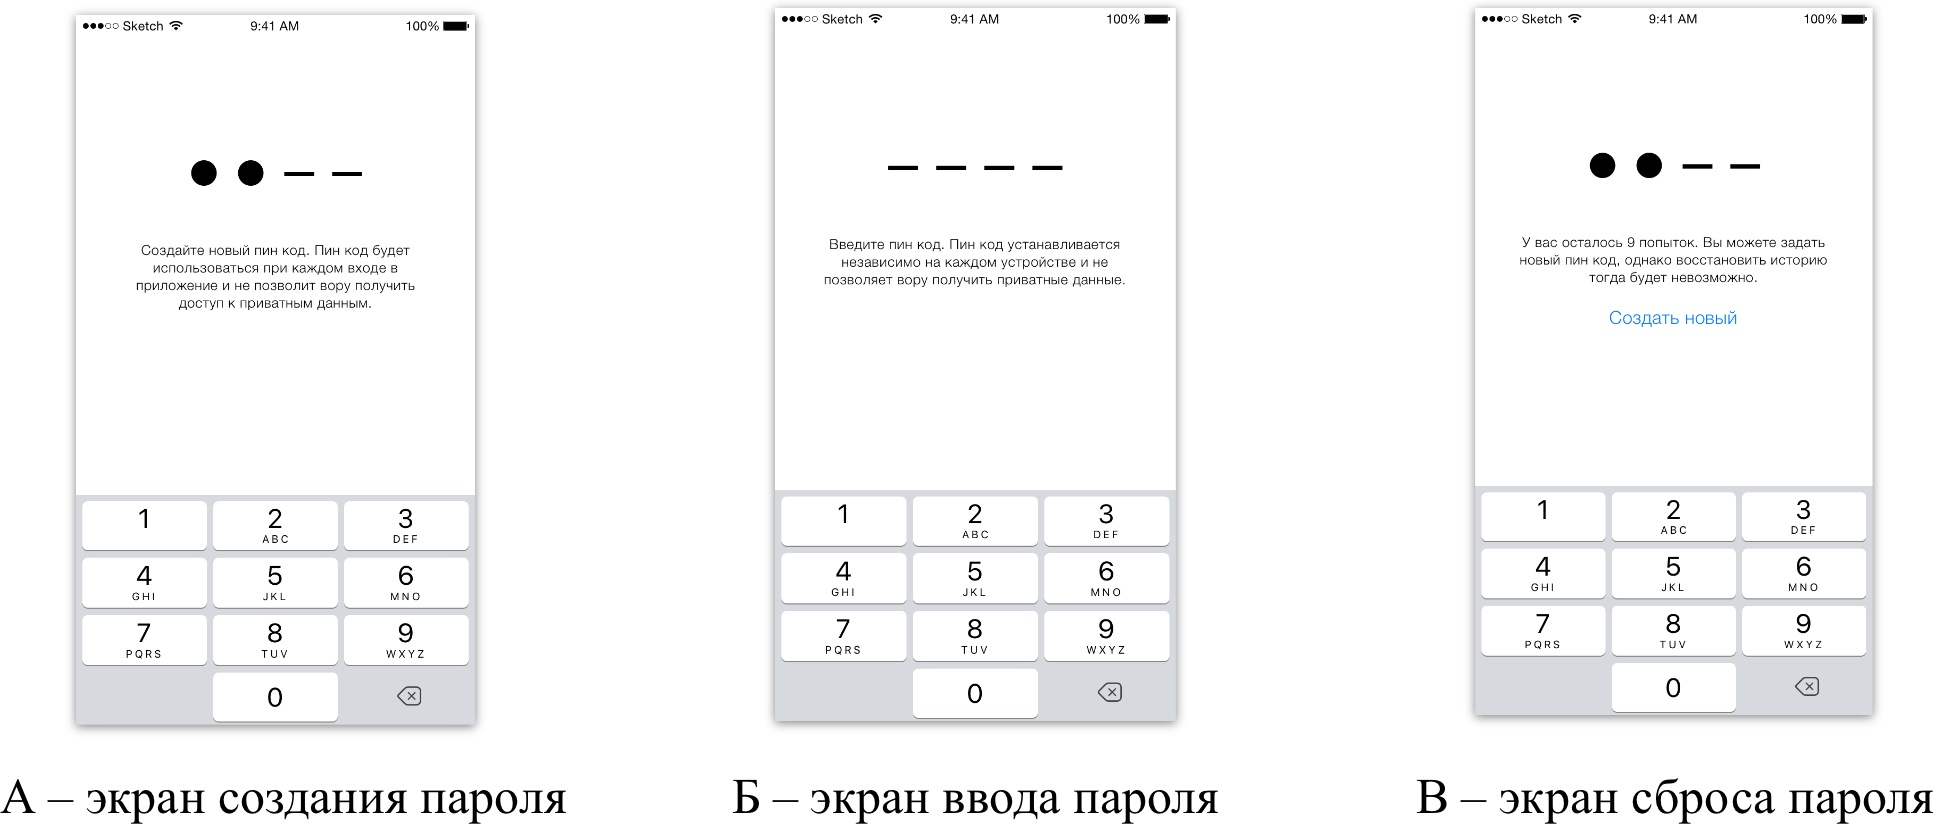
\includegraphics[width=0.75\textwidth]{inc/img/pin_combined.jpg}
  \caption{Экраны пароля клиента}
  \label{sec:usage:pin:ui}
\end{figure}

Сквозвное шифрование не способно защитить пользователя от утери или кражи устройства, что, в свою очередь, ведёт к рискам получения информации не с сервера, но с устройства. Приложение делает всё возможное для повышения безопасности хранимых локально данных и схема активации устройства через пароль клиента является одной из самых эффективных составляющих системы.